\chapter{Fondements Théoriques et Choix Technologiques}
\label{chap:fondements-techniques}

La mise en œuvre d'un système d'automatisation du processus KYC repose sur un socle théorique et technologique solide. Ce chapitre pose les bases conceptuelles nécessaires à la compréhension des choix effectués, depuis les fondements de l'intelligence artificielle et de la vision par ordinateur jusqu'aux technologies retenues. Une fois ce cadre établi, il devient possible de justifier rigoureusement la sélection des outils constituant le pipeline IA du projet.


%=============================================================
\section{Fondements théoriques}
\label{sec:fondements-theoriques}
%=============================================================

\subsection{Intelligence artificielle, machine learning et deep learning}
\label{subsec:ia-ml-dl}

Avant d'aborder la vision par ordinateur, il convient de présenter la hiérarchie conceptuelle sur laquelle elle repose. Ces trois disciplines s'emboîtent selon une relation de spécialisation croissante, chacune constituant un sous-ensemble plus restreint de la précédente.

\begin{figure}[H]
  \centering
  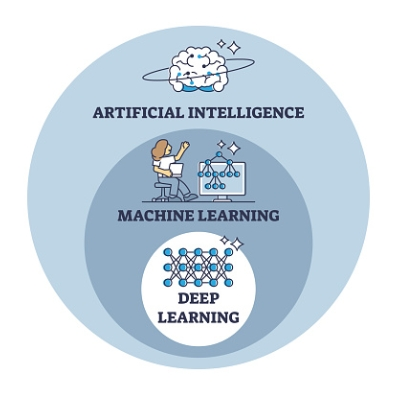
\includegraphics[width=0.75\textwidth]{images/image_chap2/ia_ml_dl.png}
  \caption{\textit{Figure 2.1 --- Relation hiérarchique entre IA, ML et Deep Learning}}
  \label{fig:ch2-ia-ml-dl}
\end{figure}

\begin{itemize}
  \item \textbf{Intelligence Artificielle (IA) :} domaine regroupant l'ensemble des techniques permettant à une machine de simuler des comportements intelligents --- apprentissage, raisonnement et prise de décision.

  \item \textbf{Machine Learning (ML) :} sous-discipline de l'IA dans laquelle les systèmes apprennent à partir de données, sans être explicitement programmés pour chaque tâche.

  \item \textbf{Deep Learning (DL) :} évolution du ML fondée sur des réseaux de neurones profonds, capables de traiter des données complexes (images, audio, texte). Le Deep Learning constitue aujourd'hui le moteur principal des systèmes de vision par ordinateur.
\end{itemize}

\subsection{Vision par ordinateur et réseaux de neurones}
\label{subsec:vision-ordinateur}

La vision par ordinateur est une branche de l'intelligence artificielle qui permet aux machines d'interpréter et de comprendre le contenu visuel d'images ou de vidéos. Son objectif est de transformer des données visuelles brutes --- des pixels --- en informations sémantiques exploitables, reproduisant ainsi de façon automatisée les capacités du système visuel humain.

Dans le cadre du KYC, la vision par ordinateur intervient à travers plusieurs applications complémentaires et étroitement liées :

\begin{itemize}
  \item \textbf{Reconnaissance d'images :} identification du type de document (carte nationale d'identité, passeport, etc.).

  \item \textbf{Détection d'objets :} localisation des zones d'intérêt --- photographie, champs textuels.

  \item \textbf{Reconnaissance optique de caractères (OCR) :} extraction et conversion du texte présent dans l'image en données numériques structurées.
\end{itemize}

Ces applications reposent sur les réseaux de neurones artificiels, brique fondamentale du Deep Learning. Inspirés du fonctionnement du cortex cérébral, ces réseaux sont composés de neurones interconnectés organisés en couches successives, chacune apprenant à extraire des représentations de plus en plus abstraites à partir des données d'entrée.

\begin{figure}[H]
  \centering
  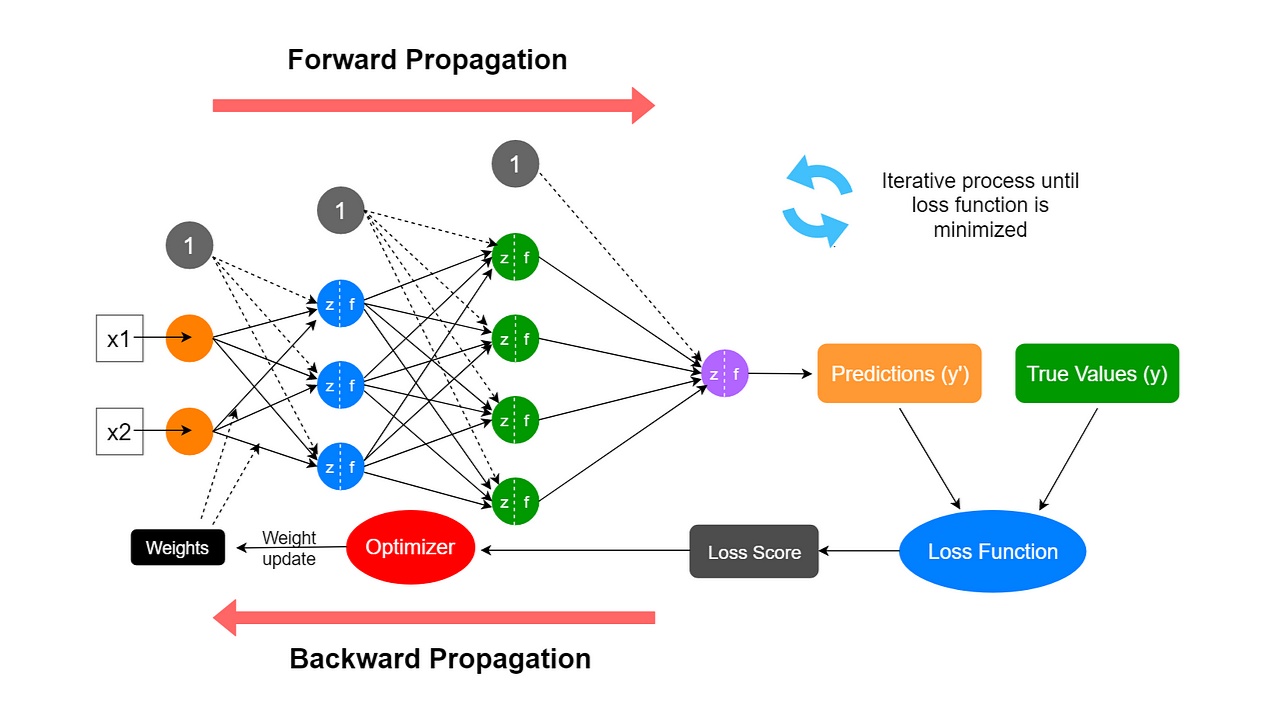
\includegraphics[width=0.75\textwidth]{images/image_chap2/1742401020360.png}
  \caption{\textit{Figure 2.2 --- Propagation avant et rétropropagation dans un réseau de neurones}}
  \label{fig:ch2-neurones}
\end{figure}

L'architecture d'un réseau de neurones se décompose en trois types de couches :

\begin{itemize}
  \item \textbf{Couche d'entrée (Input Layer) :} reçoit les données brutes --- pixels de l'image du document --- et les transmet aux couches suivantes.

  \item \textbf{Couches cachées (Hidden Layers) :} traitent l'information à travers plusieurs étapes de calcul afin d'extraire les caractéristiques complexes (contours, formes, zones de texte).

  \item \textbf{Couche de sortie (Output Layer) :} fournit la prédiction finale, telle que la probabilité qu'une zone détectée corresponde à un nom, un prénom ou un numéro de CIN.
\end{itemize}

Le fonctionnement repose sur deux phases complémentaires et itératives :

\begin{itemize}
  \item \textbf{Propagation avant (Forward Propagation) :} l'information circule de l'entrée vers la sortie pour générer une prédiction, en appliquant des poids et des biais à chaque neurone.

  \item \textbf{Rétropropagation (Backpropagation) :} le système calcule l'erreur via une fonction de perte et remonte le réseau pour ajuster les poids grâce à un optimiseur, permettant au modèle d'apprendre de ses erreurs de manière itérative.
\end{itemize}

\subsection{Détection d'objets}
\label{subsec:detection-objets}

La détection d'objets est une tâche centrale de la vision par ordinateur qui consiste à identifier et localiser simultanément plusieurs objets dans une image ou une vidéo. Contrairement à la classification d'images --- qui attribue une unique étiquette à l'ensemble de l'image --- la détection d'objets détermine la position précise de chaque objet à l'aide de boîtes englobantes (bounding boxes).

\begin{figure}[H]
  \centering
  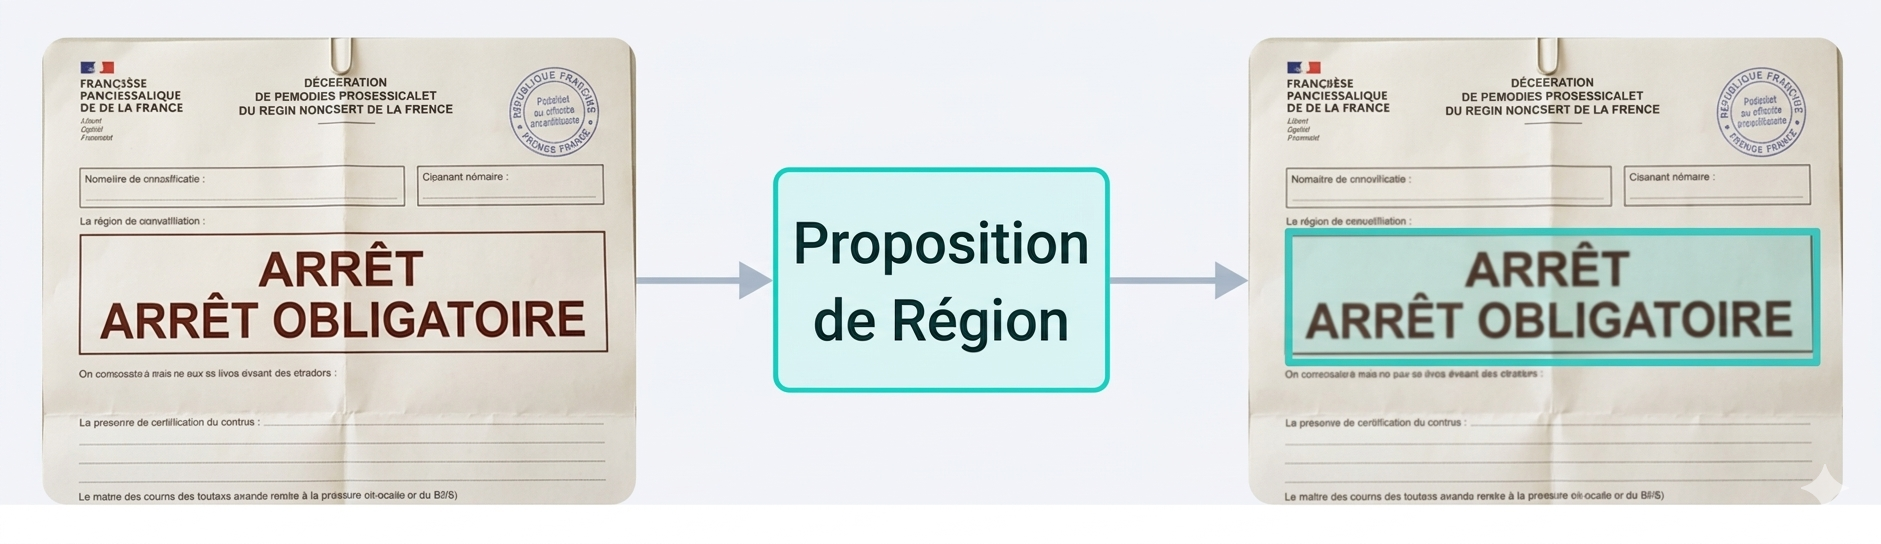
\includegraphics[width=0.75\textwidth]{images/image_chap2/detectionObjet.png}
  \caption{\textit{Figure 2.3 --- Illustration de la détection d'objets}}
  \label{fig:ch2-detection-objets}
\end{figure}

\subsubsection*{Niveaux de complexité des tâches de vision}

Pour bien situer la détection d'objets dans le spectre des tâches de vision par ordinateur, il est utile de les classer par ordre de complexité croissante :

\begin{itemize}
  \item \textbf{Classification d'image :} prédire la classe d'un objet unique dans l'image (ex. : « Ceci est une carte d'identité »).

  \item \textbf{Localisation d'objet :} identifier la présence d'un objet et indiquer sa position par une boîte englobante.

  \item \textbf{Détection d'objets :} identifier et localiser plusieurs objets et leurs classes respectives dans une même image.

  \item \textbf{Segmentation sémantique :} classifier chaque pixel de l'image dans une catégorie, sans distinguer les différentes instances d'une même classe.

  \item \textbf{Segmentation d'instance :} identifier et délimiter chaque objet distinct --- par exemple, séparer deux cartes d'identité disposées côte à côte.
\end{itemize}

\subsubsection*{Méthodes de détection : One-Stage vs Two-Stage}

Les méthodes de détection d'objets basées sur le Deep Learning se répartissent en deux grandes familles architecturales, dont le choix est guidé par le compromis entre vitesse d'inférence et précision.

\begin{figure}[H]
  \centering
  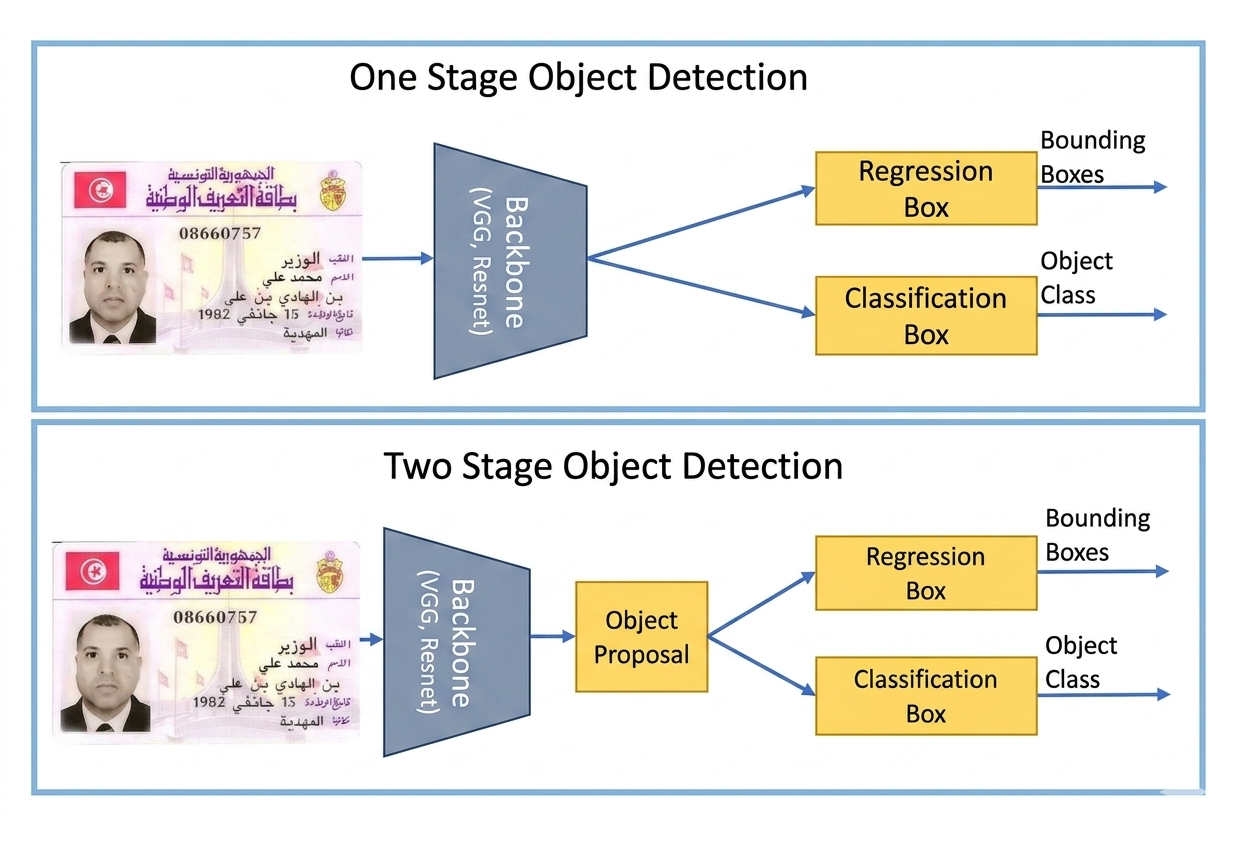
\includegraphics[width=0.45\textwidth]{images/image_chap2/onevtwoStage.png}
  \caption{\textit{Méthodes de détection d'objets : One-Stage vs Two-Stage}}
  \label{fig:ch2-one-vs-two-stage}
\end{figure}

\paragraph{Méthodes One-Stage}

Ces méthodes utilisent un réseau unique qui mappe directement l'image d'entrée vers les prédictions (boîtes englobantes et classes) en un seul passage. Leur architecture simplifiée leur confère une vitesse d'inférence élevée, idéale pour les applications en temps réel (vidéo, mobile). Exemples représentatifs : YOLO, SSD.

\paragraph{Méthodes Two-Stage}

Elles procèdent en deux étapes distinctes : une première génère des propositions de régions d'intérêt (Region Proposals), et une seconde affine et classifie ces propositions. Leur précision est généralement supérieure, au prix d'une latence plus élevée et d'un coût computationnel important. Exemples : Faster R-CNN, R-CNN.

\subsubsection*{YOLO (You Only Look Once)}

\begin{figure}[H]
  \centering
  
\includegraphics[width=0.45\textwidth]{images/image_chap2/yoloLogo.png}
  \caption{\textit{Figure 2.5 --- Logo YOLO}}
  \label{fig:ch2-yolo-logo}
\end{figure}

YOLO (You Only Look Once) est un algorithme de détection d'objets appartenant à la famille One-Stage, introduit en 2016 par Joseph Redmon et ses collaborateurs. Ce modèle a révolutionné la détection d'objets en proposant une approche unifiée, capable de détecter et classifier des objets en un seul passage réseau, atteignant des performances en temps réel tout en conservant une précision compétitive.

\paragraph{Principe de fonctionnement}
\begin{figure}[H]
  \centering
  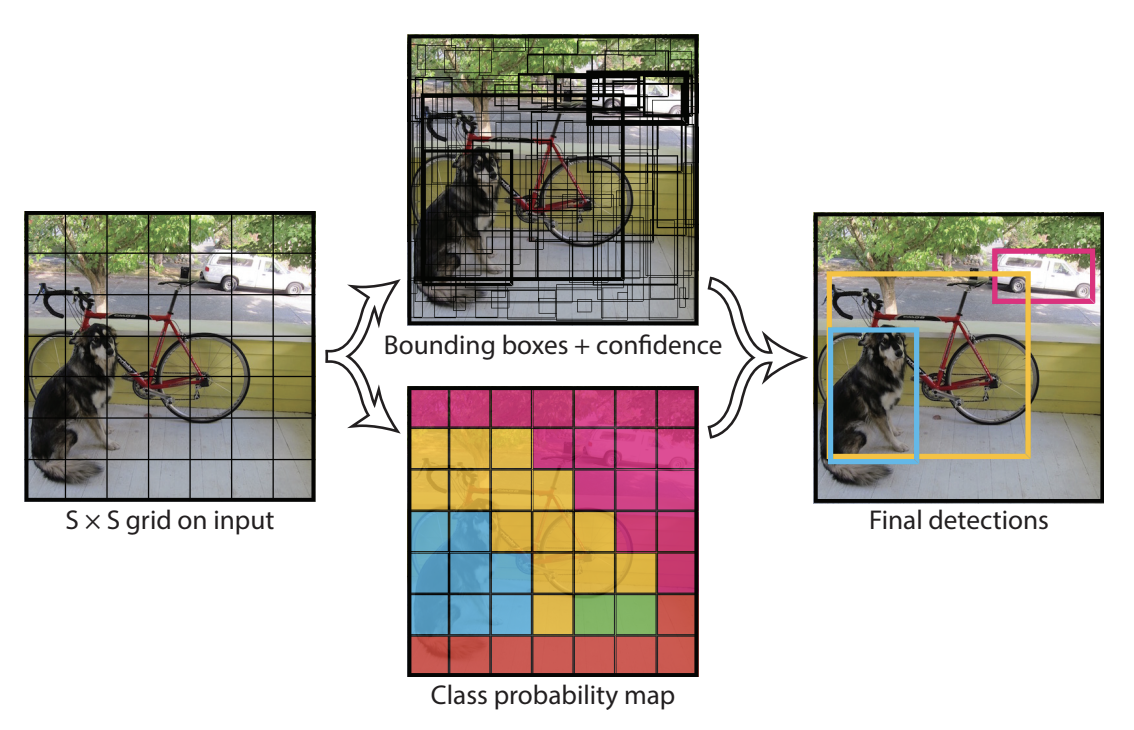
\includegraphics[width=0.75\textwidth]{images/image_chap2/detection.png}
  \caption{\textit{Principe de fonctionnement de YOLO}}
  \label{fig:Principe de fonctionnement de YOLO }
\end{figure}

Comme illustré ci-après, YOLO adopte une approche globale et unifiée :

\begin{itemize}
  \item L'image est divisée en une grille de cellules $S \times S$.
  \item Chaque cellule est responsable de la détection des objets dont le centre se situe dans sa zone.
  \item Pour chaque cellule, le modèle prédit simultanément : des boîtes englobantes, un score de confiance et la classe de l'objet.
  \item L'ensemble de ces prédictions est réalisé en un seul passage à travers le réseau, garantissant rapidité et efficacité.
\end{itemize}

\paragraph{Évolution de l'architecture YOLO}

Depuis l'introduction de YOLOv1, le modèle a connu de nombreuses itérations, chacune améliorant la précédente en termes de précision, de rapidité et d'efficacité.

\begin{figure}[H]
  \centering
  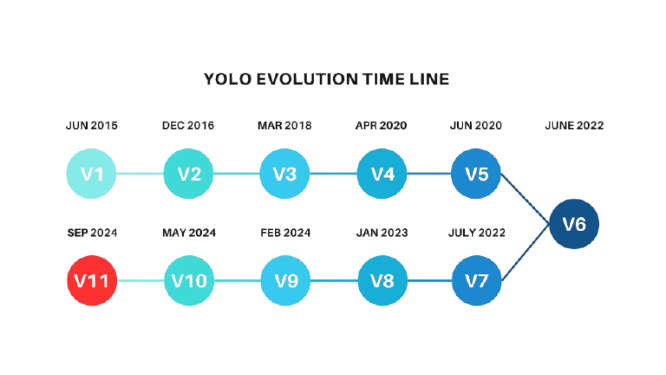
\includegraphics[width=0.90\textwidth]{images/image_chap2/TimelineCycle-removebg-preview.png}
  \caption{\textit{Figure 2.6 --- Chronologie de l'évolution des architectures YOLO (V1 à V11)}}
  \label{fig:ch2-yolo-evolution}
\end{figure}

\begin{itemize}
  \item \textbf{YOLOv1 (2016) :} modèle original --- performances temps réel, mais détection des petits objets limitée.

  \item \textbf{YOLOv2 (2017) :} introduction des boîtes d'ancrage, normalisation par lots et résolution accrue.

  \item \textbf{YOLOv3 (2018) :} prédictions multi-échelles via pyramides de features, améliorant la détection à différentes tailles d'objets.

  \item \textbf{YOLOv4 (2020) :} augmentation mosaïque et optimisation du backbone pour une inférence plus rapide.

  \item \textbf{YOLOv5 (2020) :} implémentation PyTorch largement adoptée, optimisée pour le déploiement pratique.

  \item \textbf{YOLOv6/v7 (2022) :} amélioration de la mise à l'échelle et de la précision, avec des versions compactes pour edge devices.

  \item \textbf{YOLOv8 (2023) :} backbone CSPDarkNet et agrégation de chemins améliorée, rehaussant vitesse et précision.

  \item \textbf{YOLO11 (2024) :} architecture C3K2 + SPPF + mécanisme d'attention C2PSA --- meilleure détection des petits objets et efficacité computationnelle supérieure.
\end{itemize}

\paragraph{Analyse comparative sur COCO}

\begin{figure}[H]
  \centering
  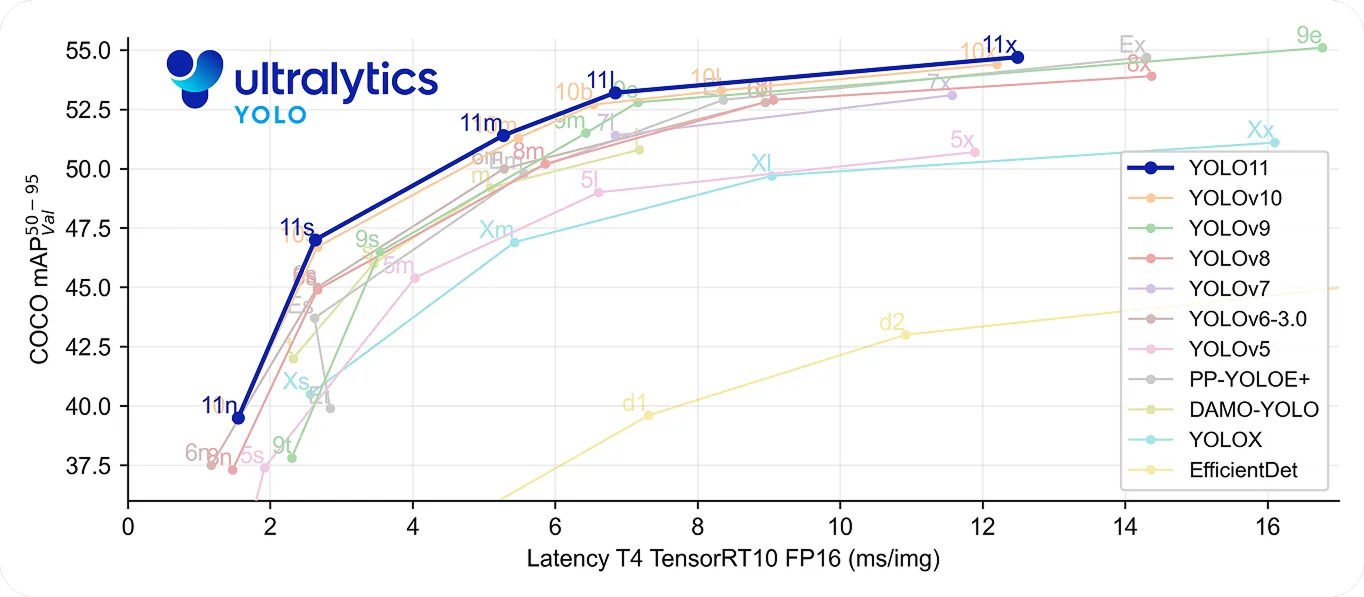
\includegraphics[width=0.75\textwidth]{images/image_chap2/Latency.png}
  \caption{\textit{Comparaison mAP50-95 / latence des modèles YOLO sur le dataset COCO}}
  \label{fig:ch2-yolo-comparaison}
\end{figure}

La figure ci-dessus compare les modèles YOLO à l'aide de la métrique mAP50-95 (mean Average Precision) sur le dataset COCO, en fonction de leur latence d'inférence. Les versions récentes offrent de meilleures performances, avec une précision accrue et une latence réduite. YOLO11 se distingue notamment par son efficacité : plus léger que ses homologues à haute précision, il conserve un excellent niveau de mAP, le rendant particulièrement adapté aux applications en temps réel.

\subsection{Reconnaissance optique de caractères (OCR)}
\label{subsec:ocr}

La reconnaissance optique de caractères (OCR --- Optical Character Recognition) est une technologie permettant d'extraire automatiquement du texte à partir d'images ou de documents numérisés. Elle transforme des informations textuelles visuelles en données numériques exploitables, facilitant leur traitement, leur stockage et leur analyse automatisée.

Dans le cadre des systèmes KYC, l'OCR joue un rôle central en permettant d'extraire les informations présentes sur les documents d'identité : nom, prénom, date de naissance, numéro d'identification, etc.

\subsubsection*{Pipeline OCR : processus pas à pas}

Le pipeline OCR se compose de cinq étapes séquentielles qui transforment une image brute en texte structuré exploitable :

\begin{figure}[H]
  \centering
  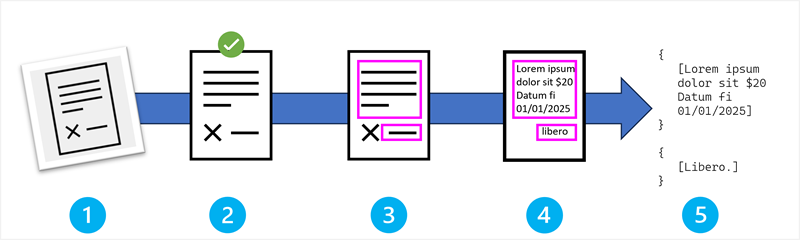
\includegraphics[width=0.75\textwidth]{images/image_chap2/optical-character-recognition.png}
  \caption{\textit{Figure 2.8 --- Pipeline OCR en cinq étapes}}
  \label{fig:ch2-ocr-pipeline}
\end{figure}

\begin{itemize}
  \item \textbf{Étape 1 --- Acquisition et entrée d'image :} le pipeline démarre à la réception de l'image. La qualité de celle-ci conditionne directement la précision finale de l'extraction de texte.

  \item \textbf{Étape 2 --- Prétraitement et amélioration :} nettoyage et optimisation de l'image pour améliorer la lisibilité.

  \item \textbf{Étape 3 --- Détection des régions textuelles :} localisation des zones contenant du texte au sein de l'image.

  \item \textbf{Étape 4 --- Reconnaissance des caractères :} identification des caractères présents dans les zones détectées.

  \item \textbf{Étape 5 --- Post-traitement et sortie :} structuration et correction des données extraites.
\end{itemize}

Ce processus permet de transformer une image contenant du texte en un format exploitable par un système informatique.

\subsubsection*{Benchmark des moteurs OCR open source}

Plusieurs solutions OCR open source ont été développées, présentant des performances variables en termes de précision, de robustesse et de vitesse. Les approches basées sur le Deep Learning, telles que PaddleOCR, se révèlent généralement plus performantes en conditions réelles (flou, bruit, faible éclairage), ce qui les rend particulièrement adaptées aux systèmes KYC.

\begin{table}[H]
  \centering
  \tiny
  \begin{tabular}{|l|c|c|c|c|c|c|c|}
    \toprule
    \rowcolor{bleu_principal}
    \textcolor{white}{\textbf{Moteur}} & \textcolor{white}{\textbf{Archi.}} & \textcolor{white}{\textbf{Préc.}} & \textcolor{white}{\textbf{CER}} & \textcolor{white}{\textbf{Vit.}} & \textcolor{white}{\textbf{Ar.}} & \textcolor{white}{\textbf{FT}} & \textcolor{white}{\textbf{Lic.}} \\
    \midrule
    Tesseract & LSTM + HMM & ~90\% & 3--5\% & Très rapide & Oui & Oui & Apache 2.0 \\
    \midrule
    \rowcolor{gris_leger}
    PaddleOCR & CNN + Transformer & ~93\% & 2--4\% & Moyen & Oui & Oui & Apache 2.0 \\
    \midrule
    EasyOCR & CRAFT + CRNN & ~85\% & 5--8\% & Lent & Oui & Partiel & Apache 2.0 \\
    \midrule
    \rowcolor{gris_leger}
    Kraken v5 & BLLA + CLSTM & ~82\% & 2--5\% & Rapide & Excellent RTL & Oui & Apache 2.0 \\
    \midrule
    MMOCR v1 & CNN / Transformer & ~84\% & 4--7\% & Moyen & Partiel & Oui & Apache 2.0 \\
    \midrule
    \rowcolor{gris_leger}
    TrOCR & ViT + BEiT & ~91\% & 2--4\% & Lent (GPU) & Non off. & Oui & MIT \\
    \bottomrule
  \end{tabular}
  \caption{Benchmark des principaux moteurs OCR open source (mise à jour 2025)}
  \label{tab:ocr-benchmark}
\end{table}

Les scores de précision sont des moyennes indicatives sur texte imprimé propre (300 DPI+). Le CER (Character Error Rate) varie significativement selon la qualité du scan, la langue et le domaine. PP-OCRv5 est à ce jour le seul moteur à combiner support natif de l'arabe (RTL), fine-tuning aisé et analyse de mise en page avancée.


%=============================================================
\section{Choix technologiques}
\label{sec:choix-technologiques}
%=============================================================

Les fondements théoriques présentés précédemment guident naturellement vers la sélection des outils les plus adaptés au contexte du projet. Deux technologies ont été retenues après une analyse comparative rigoureuse : YOLO11m pour la détection d'objets et PP-OCRv5 pour la reconnaissance de caractères.

\subsection{Modèle de détection : YOLO11m}
\label{subsec:yolo11m}

\subsubsection*{Présentation de YOLO11}

YOLO11 est la dernière génération de modèles de détection d'objets en temps réel développée par Ultralytics, publiée en septembre 2024. Il introduit plusieurs innovations architecturales majeures par rapport à ses prédécesseurs :

\begin{itemize}
  \item \textbf{Bloc C3K2 (Cross Stage Partial with Kernel Size 2) :} extraction de caractéristiques spatiales plus riche.

  \item \textbf{Module SPPF (Spatial Pyramid Pooling Fast) :} meilleure capture multi-échelle des objets de différentes tailles.

  \item \textbf{Bloc C2PSA (Convolutional with Parallel Spatial Attention) :} amélioration de la détection des petits objets.
\end{itemize}

La famille YOLO11 propose cinq variantes (n, s, m, l, x) couvrant un spectre allant des dispositifs embarqués aux serveurs GPU haute performance.

\subsubsection*{Comparaison des variantes YOLO11}

Le tableau suivant présente les performances benchmarkées sur le dataset COCO (mAP50-95) pour chaque variante, en précisant le nombre de paramètres et la vitesse d'inférence CPU.

\begin{table}[H]
  \centering
  \begin{tabular}{|l|c|c|c|c|l|}
    \toprule
    \rowcolor{bleu_principal}
    \textcolor{white}{\textbf{Variante}} & \textcolor{white}{\textbf{Paramètres}} & \textcolor{white}{\textbf{GFLOPs}} & \textcolor{white}{\textbf{mAP}} & \textcolor{white}{\textbf{CPU (ms)}} & \textcolor{white}{\textbf{Usage}} \\
    \midrule
    YOLO11n & 2,6 M & 6,5 & 39,5\% & 56,1 & Edge / mobile \\
    \midrule
    \rowcolor{gris_leger}
    YOLO11s & 9,4 M & 21,5 & 47,0\% & 90,0 & Léger temps réel \\
    \midrule
    \textbf{YOLO11m} & \textbf{20,1 M} & \textbf{68,0} & \textbf{51,5\%} & \textbf{183,2} & \textbf{Équilibre optimal} \\
    \midrule
    \rowcolor{gris_leger}
    YOLO11l & 25,3 M & 86,9 & 53,4\% & 232,6 & Haute précision \\
    \midrule
    YOLO11x & 56,9 M & 194,9 & 54,7\% & 462,8 & Précision maximale \\
    \bottomrule
  \end{tabular}
  \caption{Comparaison des variantes YOLO11 sur COCO val2017}
  \label{tab:yolo11-variantes}
\end{table}

La variante YOLO11m offre le meilleur équilibre entre précision et complexité computationnelle pour notre contexte d'application. Les variantes légères (n, s) privilégient la vitesse au détriment de la précision, tandis que les modèles lourds (l, x) engendrent des coûts incompatibles avec les contraintes d'un système bancaire opérationnel.

\subsubsection*{Justification du choix : YOLO11m vs YOLOv8m}

Le tableau ci-dessous compare YOLO11m à YOLOv8m, qui constitue la génération précédente la plus répandue en production.

\begin{table}[H]
  \centering
  \small
  \begin{tabular}{|l|c|c|c|}
    \toprule
    \rowcolor{bleu_principal}
    \textcolor{white}{\textbf{Critère}} & \textcolor{white}{\textbf{YOLO11m}} & \textcolor{white}{\textbf{YOLOv8m}} & \textcolor{white}{\textbf{Avantage}} \\
    \midrule
    Paramètres & 20,1 M & 25,9 M & $-$22\% (YOLO11m) \\
    \midrule
    \rowcolor{gris_leger}
    mAP50-95 (COCO) & 51,5\% & 50,2\% & +1,3 pt (YOLO11m) \\
    \midrule
    Vitesse CPU (ms) & 183,2 & $\sim$220 & Plus rapide \\
    \midrule
    \rowcolor{gris_leger}
    Architecture & C3K2 + SPPF + C2PSA & C2f + SPPF & Extraction enrichie \\
    \midrule
    Déploiement & Edge / Cloud / GPU & Edge / Cloud / GPU & Équivalent \\
    \bottomrule
  \end{tabular}
  \caption{YOLO11m vs YOLOv8m : gains en précision et efficacité}
  \label{tab:yolo11-vs-yolov8}
\end{table}

YOLO11m a été retenu car il offre le meilleur compromis entre précision (mAP 51,5\%) et coût computationnel, tout en nécessitant 22\% de paramètres en moins que YOLOv8m. Cette légèreté le rend plus adapté à une intégration dans un système bancaire contraint en ressources matérielles.

\subsection{Moteur OCR : PaddleOCR PP-OCRv5}
\label{subsec:pp-ocrv5}

\subsubsection*{Présentation de PP-OCRv5}

PP-OCRv5 est la cinquième génération du pipeline OCR de PaddlePaddle (Baidu), publiée dans le cadre de PaddleOCR 3.0 en 2024. Il représente une évolution majeure conçue spécifiquement pour la reconnaissance de texte dans des environnements variés et multilingues, incluant des documents réels, du texte manuscrit et des images capturées en conditions non contrôlées.

L'architecture repose sur un pipeline à deux étages : détection des zones de texte (PP-OCRv5\_det), puis reconnaissance caractère par caractère (PP-OCRv5\_rec), disponible en variante mobile (optimisée CPU) et serveur (optimisée GPU).

\subsubsection*{Performances et évolution par rapport aux versions précédentes}

\begin{table}[H]
  \centering
  \small
  \begin{tabular}{|l|c|c|c|}
    \toprule
    \rowcolor{bleu_principal}
    \textcolor{white}{\textbf{Critère}} & \textcolor{white}{\textbf{PP-OCRv3}} & \textcolor{white}{\textbf{PP-OCRv4}} & \textcolor{white}{\textbf{PP-OCRv5}} \\
    \midrule
    Langues supportées & 80+ & 80+ & 106 (arabe inclus) \\
    \midrule
    \rowcolor{gris_leger}
    Amélioration précision & Référence & +10--15\% & +30\% multi / +13 pts \\
    \midrule
    Support arabe & Partiel & Partiel & Natif (2\,676 img) \\
    \midrule
    \rowcolor{gris_leger}
    Texte déformé / incliné & Limité & Moyen & Amélioré \\
    \midrule
    Variantes & Mobile seul & Mobile + Server & Mobile + Server \\
    \midrule
    \rowcolor{gris_leger}
    Performance vs VLM & --- & --- & Surpasse GPT-4o, Gemini \\
    \bottomrule
  \end{tabular}
  \caption{Évolution des performances PP-OCR à travers les versions}
  \label{tab:pp-ocr-evolution}
\end{table}

\subsubsection*{Critères de sélection pour le contexte tunisien}

Le choix de PP-OCRv5 s'appuie sur quatre critères directement liés aux contraintes du projet KYC de la BTE.

\paragraph{a) Support natif de l'arabe}

PP-OCRv5 couvre 106 langues, dont l'arabe, le français et l'anglais, avec un dataset arabe dédié de 2\,676 images d'entraînement. L'arabe étant une langue à écriture cursive et de droite à gauche (RTL), la majorité des solutions OCR classiques échouent sur ce type de texte. PP-OCRv5 intègre nativement cette complexité, le rendant parfaitement adapté aux documents d'identité tunisiens bilingues (arabe / français).

\paragraph{b) Amélioration de précision documentée}

Comparé à PP-OCRv3, PP-OCRv5 atteint une amélioration de plus de 30\% en précision pour la reconnaissance multilingue, et +13 points de pourcentage d'amélioration globale par rapport à PP-OCRv4. Ces gains sont particulièrement significatifs sur les scénarios de texte déformé, incliné ou manuscrit --- conditions précisément rencontrées lors de la capture mobile d'images KYC.

\paragraph{c) Performance face aux grands modèles de vision (VLM)}

Dans les benchmarks publiés sur OmniDocBench, PP-OCRv5 surpasse des modèles de grande taille tels que GPT-4o, Gemini 2.5 Pro et Qwen2.5-VL sur les tâches OCR spécialisées, tout en utilisant moins de 100 millions de paramètres. Cette efficacité est essentielle pour un déploiement on-premise dans un environnement bancaire aux ressources définies.

\paragraph{d) Licence open source et facilité d'intégration}

PP-OCRv5 est distribué sous licence Apache 2.0, sans restriction commerciale. Il dispose d'une API Python claire et d'une intégration native avec PaddlePaddle 3.0, permettant une incorporation directe dans le pipeline KYC de la banque, sans dépendance à des services cloud tiers.

\vspace{0.5cm}

PP-OCRv5 représente à ce jour l'une des rares solutions open source capables de traiter de manière robuste des documents bilingues arabe/français dans des conditions réelles de capture mobile --- ce qui constitue précisément le défi central du projet KYC de la BTE.


\section*{Conclusion du chapitre}

Ce chapitre a établi les fondements théoriques et technologiques du système. L'ancrage dans les principes de l'IA, du Deep Learning et de la vision par ordinateur a permis de justifier rigoureusement le choix de YOLO11m pour la détection d'objets et de PP-OCRv5 pour la reconnaissance de texte arabe et français. Ces deux briques technologiques forment le socle sur lequel s'appuie l'implémentation du pipeline IA décrite dans le chapitre suivant.
